\documentclass[11pt, a4paper]{article}
\usepackage{CJKutf8}
\usepackage{amsthm}
\usepackage{ulem}
\usepackage{xcolor}
\usepackage{amsmath}
\usepackage{multicol}
\usepackage{amssymb}
\usepackage{courier}
\usepackage{geometry}
\usepackage{enumitem}
\usepackage{graphicx}
\usepackage{subfigure}
\usepackage{listings}
\usepackage{algorithm}
\usepackage{algorithmic}
\usepackage{indentfirst}
\usepackage{amsmath}
\DeclareMathOperator*{\argmax}{arg\,max}
\usepackage[perpage,stable]{footmisc} 
\geometry{left=2.7cm, right=2.7cm, top=3cm, bottom=3cm}

\lstset{numbers=left, language=C++,basicstyle=\ttfamily\small,frame=shadowbox,
	keywordstyle=\color{blue!70}, commentstyle=\color{red!50!green!50!blue!50},
	escapeinside='',extendedchars=false}

\usepackage[colorlinks,linkcolor=black,anchorcolor=blue,citecolor=green,
%	CJKbookmarks=true,
]{hyperref}
\hypersetup{unicode}


\linespread{1.4}

\begin{document}
	\begin{CJK*}{UTF8}{gbsn}
		
		\title{\bf 大作业报告}
		\author{文灏洋}
		\date{}
		\maketitle
		\setlength{\parindent}{2em}
		\renewcommand{\contentsname}{\textbf{目录}}
		\tableofcontents
				
		\newpage
		\section{中文分词}
			词是中文的最小表意单位,而英文之间有空格来区分单词与单词,中文却没有明显的词语的区分,所以中文分词旨在将一个汉字序列切分成一个个独立的词。
		\section{算法}
				\newtheorem*{theorem}{问题描述}

			\subsection{问题的形式化定义}
					\begin{theorem}
						对于每一个句子 $x$ ,找出一个可能的按词分隔好的句子 $F(x)$ ,满足
							 \begin{equation*}
								 F(x) = \argmax_{y\in GEN(x)} Score(y)
							 \end{equation*}
					\end{theorem}
				
			\subsection{转化为序列标注问题}
				将中文分词转化为序列标注问题的办法利用BMES四个标记来标记每一个字,其中B表示这个字在词语中是词首,M表示词中,E表示词尾,S表示单字成词。
				这样就转变成了
					\begin{theorem}
						 给定一段中文序列T,找出标记序列
						 \begin{equation*}
						 O = \argmax_{O}{Score(O|T)}
						 \end{equation*} 
					\end{theorem}
			\subsection{Perceptron分类器}
				我采用了感知机分类器将词性标注建模为对单个词的上下文环境进行分类。
				对一个字 $w_i$ ,其选择其特征为下表:
				\begin{multicols}{3}
						\begin{itemize}
							\item $w_{i - 2}$
							\item $w_{i - 1}$
							\item $w_i$
							\item $w_{i + 1}$
							\item $w_{i + 2}$
							\item $(w_{i - 2},w_{i - 1})$
							\item $(w_{i - 1},w_i)$
							\item $(w_{i},w_{i + 1})$
							\item $(w_{i + 1},w_{i + 2})$
							\item $O_{i - 1}$
						\end{itemize}
				\end{multicols}
				这样,$w_i$ 采用标记 $tag$ 的权重即为
				\begin{equation*}
					Score(tag) = \Phi(w_i) \cdot \overline{\alpha_{tag}}
				\end{equation*}
				我们就可以选择权重最大的作为该字的标记
				\subsubsection{训练}
					训练采用常规的感知机的训练方法,伪代码如下:
					\begin{algorithm}
						\caption{Training}               %标题
						\label{alg1}                         %标记算法,方便在其它地方引用
						\begin{algorithmic}
							\FORALL {$tag$}
								\STATE $\overline{\alpha_{tag}}\leftarrow \vec{0}$
							\ENDFOR
							\FOR {$t = 1...T$}
								\FOR {$i = 1...N$}
									\STATE $z_i \leftarrow \argmax_{tag}{\Phi(w_i)\cdot\overline{\alpha_{tag}}}$
									\IF {$z_i \neq y_i$}
										\STATE $\overline{\alpha_{z_i}} = \overline{\alpha_{z_i}} - \Phi(w_i)$
										\STATE $\overline{\alpha_{y_i}} = \overline{\alpha_{y_i}} + \Phi(w_i)$
									\ENDIF
								\ENDFOR
							\ENDFOR
						\end{algorithmic}
					\end{algorithm}	
				\subsubsection{解码}
					由于选择的特征无后效性,所以可以采用Viterbi解码,伪代码如下:
					\begin{algorithm}
						\caption{Decoding}               %标题
						\label{alg2}                         %标记算法,方便在其它地方引用
						\begin{algorithmic}
							\FOR {$i = 1... N$}
								\FOR {$j = 1...T$}
									\FOR {$k = 1...T$}
										\IF {$score_{i,j} < score_{i-1,k} + \Phi(w_i) \cdot \overline{\alpha_{z_i}}$}
											\STATE $score_{i,j} = score_{i-1,k} + \Phi(w_i) \cdot \overline{\alpha_{z_i}}$
											\STATE $path_{i,j} = k$
										\ENDIF
									\ENDFOR
								\ENDFOR
							\ENDFOR
						\end{algorithmic}
					\end{algorithm}	
		\section{实验}
			\subsection{训练数据}
				训练数据使用的是cip-data.train,用上述的感知机算法迭代训练10次。
				最后训练出的特征一共有303870个。
			\subsection{评价方法}
				设算法分词结果的词的集合为$A$,正确结果的词的集合为$B$,
				正确率可以评价为
				\begin{eqnarray*}
					p &=& \frac{|A\cup B|}{|A|}\\q &= &\frac{|A\cup B|}{|B|}\\
					accuracy &=& \frac{2\cdot p\cdot q}{p + q}
				\end{eqnarray*}
				
				即并集的集合大小占两个集合比率的调和平均数。
				
				这也是提供的eval.py的实现方法。
			\subsection{准确率}
				\begin{figure} 
					\centering
					\subfigure[Result 1]{
						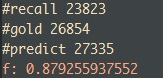
\includegraphics{result1.jpg}
						\label{g1}
					}
					\subfigure[Result 2]{
						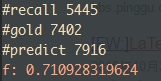
\includegraphics{result2.jpg}
						\label{g2}					
					}
				\end{figure}
				(a),(b)两图的结果是在利用训练数据cip-data.train训练,在开发数据1——judge.data.1和开发数据2——judge.data.2上跑出的结果。
				
				其中开发数据1的准确率不算太差,但是2的准确率比较差,其原因是感知机对于训练数据2中的网站的训练不够充分。
				
				所以在最终生成的结果中,我的训练数据加入了开发数据2的标准答案以训练网址的分词结果。
				
				最终生成的结果的两个文件分别为final-result-1.txt和final-result-2.txt。
		\section{其他说明}
		
			CWS文件夹内有三个文件,分别为perceptron.py,perceptron\_viterbi.py和other.py,在这里做一下说明。
			
			第一个文件采用的是上文提到的感知机训练,但是解码是采用的直接贪心。
			
			第二个文件采用的就是完整的报告提出的思路。
			
			第三个文件是直接提取少数特征(与上文提到的特征不同)在训练集中的概率分布,用Viterbi解码。
			
	\newpage			
	\end{CJK*}

\end{document}
